\documentclass[UTF8,fontset=none,12pt]{ctexart}

\setCJKmainfont{Songti SC}
\setCJKsansfont{PingFang SC}
\setCJKmonofont{Songti SC}

\usepackage[a4paper,margin=2.35cm]{geometry}
\usepackage{amsmath,amssymb,amsthm,mathtools,bm}
\usepackage{graphicx}
\usepackage{float}
\usepackage{booktabs}
\usepackage{enumitem}
\usepackage[hidelinks]{hyperref}

\newcommand{\C}{\mathbb{C}}
\newcommand{\R}{\mathbb{R}}
\newcommand{\range}{\operatorname{range}}
\newcommand{\rank}{\operatorname{rank}}
\newcommand{\Gammafun}{\mathop{\Gamma}}
\theoremstyle{definition}
\newtheorem{theorem}{定理}
\renewcommand{\thetheorem}{11.\arabic{theorem}}

\title{数值线性代数\quad 第 11 讲：最小二乘问题}
\author{Lloyd N. Trefethen、David Bau III\quad 中文阅读版}
\date{}

\begin{document}
\maketitle
\pagestyle{plain}

自高斯和勒让德在 1800 年前后发明最小二乘法以来，最小二乘数据拟合一直是不可或缺的工具，并且影响遍及数学科学的许多领域.用线性代数的语言说，本讲要处理的是超定方程组 $Ax=b$：矩阵是长方形的，行数多于列数.最小二乘的思想，是通过最小化残差 $b-Ax$ 的 2-范数来“求解”这样的系统.

\section*{问题}

考虑一个含有 $n$ 个未知数、但有 $m>n$ 个方程的线性方程组.我们希望找到满足 $Ax=b$ 的向量 $x\in\C^n$，其中
\[
    A\in\C^{m\times n},\qquad b\in\C^m.
\]
一般而言，这样的方程组没有解.只有当 $b\in\range(A)$ 时才存在合适的 $x$；而 $b$ 是 $m$ 维向量，$\range(A)$ 的维数至多为 $n$，所以这只会对特殊的 $b$ 发生.当 $m>n$ 时，这样的长方形方程组称为\textbf{超定}方程组.

把
\begin{equation}
    r=b-Ax\in\C^m
    \tag{11.1}
\end{equation}
称为\textbf{残差}.通过选择合适的 $x$，残差通常可以变得很小，但一般无法严格变成零.

如果一个没有解的问题仍要谈“求解”，这意味着什么？对超定方程组，一个自然的答案是：既然不能让残差 $r$ 等于零，就让它尽可能小.要衡量“小”，需要先选择范数.如果选择 2-范数，问题就成为：
\begin{equation}
\begin{aligned}
&\text{给定 }A\in\C^{m\times n},\quad m\ge n,\quad b\in\C^m,\\
&\text{寻找 }x\in\C^n,\quad\text{使 }\|b-Ax\|_2\text{ 最小}.
\end{aligned}
\tag{11.2}
\end{equation}
这就是一般的（线性）最小二乘问题.选择 2-范数可以由几何和统计方面的多种理由来支持；正如后面将看到的，它还会导出简单的算法，根本原因在于：二次函数的导数是线性的，而求极小值必须令导数为零.

2-范数对应欧氏距离，因此式 (11.2) 有一个直观的几何解释：寻找 $x\in\C^n$，使得 $Ax\in\C^m$ 是 $\range(A)$ 中距离 $b$ 最近的点.

\section*{例：多项式数据拟合}

下面比较两种做法：多项式插值会导出方阵方程组；最小二乘多项式数据拟合则使用长方形方程组.

\subsection*{例 11.1：多项式插值}

设给定 $m$ 个互异的点 $x_1,\ldots,x_m\in\C$，以及这些点上的数据 $y_1,\ldots,y_m\in\C$.存在唯一的多项式插值函数，即次数至多为 $m-1$ 的多项式
\begin{equation}
    p(x)=c_0+c_1x+\cdots+c_{m-1}x^{m-1},
    \tag{11.3}
\end{equation}
满足每个 $x_i$ 都有 $p(x_i)=y_i$.数据 $\{x_i\},\{y_i\}$ 与系数 $\{c_i\}$ 的关系，可由例 1.1 中已经见过的方形 Vandermonde 系统表示：
\begin{equation}
\begin{bmatrix}
1&x_1&x_1^2&\cdots&x_1^{m-1}\\
1&x_2&x_2^2&\cdots&x_2^{m-1}\\
1&x_3&x_3^2&\cdots&x_3^{m-1}\\
\vdots&\vdots&\vdots&&\vdots\\
1&x_m&x_m^2&\cdots&x_m^{m-1}
\end{bmatrix}
\begin{bmatrix}
c_0\\c_1\\c_2\\\vdots\\c_{m-1}
\end{bmatrix}
=
\begin{bmatrix}
y_1\\y_2\\y_3\\\vdots\\y_m
\end{bmatrix}.
\tag{11.4}
\end{equation}
只要点 $\{x_i\}$ 互异，这个方程组就保证非奇异，因此可以求出给定数据对应的系数（见习题 37.3）.

图~\ref{fig:11-1} 给出了一个多项式插值的例子：有 11 个数据点，它们构成一个离散的方波，用叉号表示；曲线 $p(x)$ 必须经过所有这些点.但这个拟合并不令人满意.在区间两端，$p(x)$ 出现很大的振荡，这显然是插值过程产生的伪影，而不是数据的合理反映.

\begin{figure}[H]
    \centering
    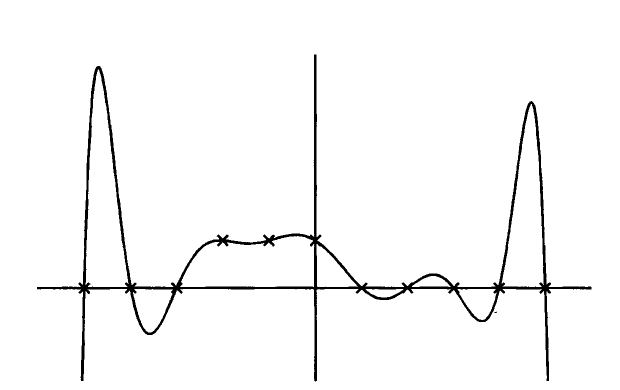
\includegraphics[width=0.78\linewidth]{../assets/figure-11-1.png}
    \caption{11 个数据点的 10 次多项式插值.图中不标出坐标轴刻度，因为刻度不会影响所要表达的形状.}
    \label{fig:11-1}
\end{figure}

这种不理想的行为是多项式插值的典型特征.它产生的拟合往往很差；使用更多数据时，情况还可能变得更糟.即使拟合看起来不错，插值过程也可能是病态的，也就是对数据扰动敏感（下一讲会讨论）.为了避免这些问题，可以在区间 $[-1,1]$ 中使用非均匀的插值点，例如 Chebyshev 点.但是在实际应用中，我们未必能随意选择插值点.

\subsection*{例 11.2：多项式最小二乘拟合}

不改变数据点，只降低多项式的次数，通常就能得到更好的结果.仍给定 $x_1,\ldots,x_m$ 和 $y_1,\ldots,y_m$，现在考虑某个 $n<m$ 的 $n-1$ 次多项式
\begin{equation}
    p(x)=c_0+c_1x+\cdots+c_{n-1}x^{n-1}.
    \tag{11.5}
\end{equation}
如果它能使数据偏差平方和
\begin{equation}
    \sum_{i=1}^{m}|p(x_i)-y_i|^2
\tag{11.6}
\end{equation}
最小，那么这个多项式就是数据的最小二乘拟合.

这个平方和等于长方形 Vandermonde 系统残差 2-范数的平方：
\begin{equation}
\begin{bmatrix}
1&x_1&\cdots&x_1^{n-1}\\
1&x_2&\cdots&x_2^{n-1}\\
1&x_3&\cdots&x_3^{n-1}\\
\vdots&\vdots&&\vdots\\
1&x_m&\cdots&x_m^{n-1}
\end{bmatrix}
\begin{bmatrix}
c_0\\c_1\\\vdots\\c_{n-1}
\end{bmatrix}
\approx
\begin{bmatrix}
y_1\\y_2\\y_3\\\vdots\\y_m
\end{bmatrix}.
\tag{11.7}
\end{equation}

图~\ref{fig:11-2} 展示了把上一个例子的 11 个数据点用 7 次多项式拟合时的结果.新的多项式不再插值通过每个数据点，但例 11.1 的多项式更好地捕捉了数据的整体趋势.虽然图中看不出来，它对扰动也更不敏感.

\begin{figure}[H]
    \centering
    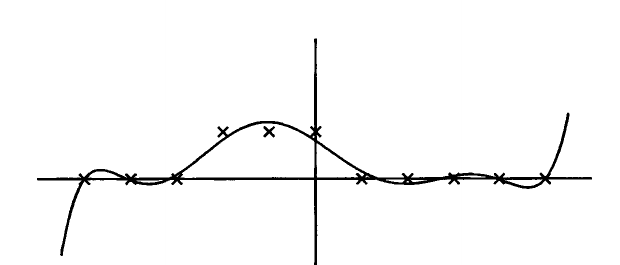
\includegraphics[width=0.78\linewidth]{../assets/figure-11-2.png}
    \caption{同一组 11 个数据点的 7 次多项式最小二乘拟合.}
    \label{fig:11-2}
\end{figure}

\section*{正交投影与正规方程}

图~\ref{fig:11-3} 说明了式 (11.2) 的几何含义.我们的目标是在 $\range(A)$ 中寻找距离 $b$ 最近的点 $Ax$，使残差 $r=b-Ax$ 的范数最小.从几何上看，只要
\[
    Ax=Pb,
\]
其中 $P\in\C^{m\times m}$ 是把 $\C^m$ 映到 $\range(A)$ 的正交投影，就能达到这个目标.换言之，残差 $r=b-Ax$ 必须与 $\range(A)$ 正交.这可以表述为下面的定理.

\begin{figure}[H]
    \centering
    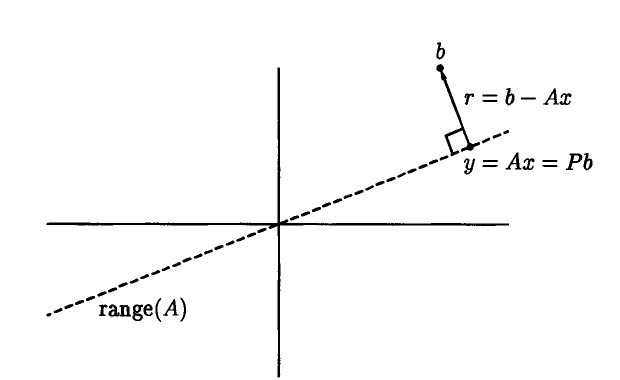
\includegraphics[width=0.78\linewidth]{../assets/figure-11-3.png}
    \caption{用正交投影表述最小二乘问题 (11.2).}
    \label{fig:11-3}
\end{figure}

\begin{theorem}
设 $A\in\C^{m\times n}$（$m\ge n$）和 $b\in\C^m$ 给定.向量 $x\in\C^n$ 最小化残差范数
\[
    \|r\|_2=\|b-Ax\|_2,
\]
从而解决最小二乘问题 (11.2)，当且仅当 $r\perp\range(A)$，也就是
\begin{equation}
    A^*r=0.
    \tag{11.8}
\end{equation}
等价地，
\begin{equation}
    A^*Ax=A^*b,
    \tag{11.9}
\end{equation}
或者
\begin{equation}
    Pb=Ax,
    \tag{11.10}
\end{equation}
其中 $P\in\C^{m\times m}$ 是到 $\range(A)$ 上的正交投影.式 (11.9) 所对应的 $n\times n$ 方程组称为\textbf{正规方程}.它非奇异，当且仅当 $A$ 满列秩.因此，最小二乘解唯一，当且仅当 $A$ 满列秩.
\end{theorem}

\paragraph{证明.}式 (11.8) 与式 (11.10) 的等价性来自第 6 讲讨论的正交投影性质；式 (11.8) 与式 (11.9) 的等价性来自残差 $r$ 的定义.

要说明 $y=Pb$ 是 $\range(A)$ 中唯一的最小化 $\|b-y\|_2$ 的点，设 $z\ne y$ 是 $\range(A)$ 中的另一个点.由于 $z-y$ 与 $b-y$ 正交，勾股定理（习题 2.2）给出
\[
    \|b-z\|_2^2=\|b-y\|_2^2+\|y-z\|_2^2>\|b-y\|_2^2,
\]
这正是所需结论.

最后，如果 $A^*A$ 奇异，那么存在非零 $x$ 使 $A^*Ax=0$.左乘 $x^*$ 得
\[
    x^*A^*Ax=\|Ax\|_2^2=0,
\]
因此 $Ax=0$，说明 $A$ 秩亏.反过来，如果 $A$ 秩亏，那么存在非零 $x$ 使 $Ax=0$，于是也有 $A^*Ax=0$，所以 $A^*A$ 奇异.结合式 (11.9)，就得到关于 $A^*A$ 非奇异性与最小二乘解唯一性的结论.\qed

\section*{伪逆}

刚才已经看到，如果 $A$ 满列秩，那么最小二乘问题 (11.2) 的解唯一，并且
\[
    x=(A^*A)^{-1}A^*b.
\]
矩阵
\begin{equation}
    A^+=(A^*A)^{-1}A^*\in\C^{n\times m}
    \tag{11.11}
\end{equation}
称为 $A$ 的\textbf{伪逆}.它把 $b\in\C^m$ 映射为 $x\in\C^n$，这也解释了为什么它的尺寸是 $n\times m$，即列数多于行数.

满列秩线性最小二乘问题 (11.2) 可以概括为：要计算下面两个向量中的一个或两个：
\begin{equation}
    x=A^+b,\qquad y=Pb.
    \tag{11.12}
\end{equation}
其中 $A^+$ 是 $A$ 的伪逆，$P$ 是到 $\range(A)$ 上的正交投影.下面介绍计算它们的三种主要算法.

\section*{正规方程}

求解最小二乘问题的经典方法，是直接求解正规方程 (11.9).如果 $A$ 满列秩，这是一组 $n\times n$ 的 Hermitian 正定方程.求解这类系统的标准方法是 Cholesky 分解，第 23 讲将讨论它.该方法构造
\[
    A^*A=R^*R,
\]
其中 $R$ 是上三角矩阵，从而把式 (11.9) 化为
\begin{equation}
    R^*Rx=A^*b.
    \tag{11.13}
\end{equation}

\subsection*{算法 11.1：通过正规方程求解最小二乘问题}

\begin{enumerate}
    \item 构造矩阵 $A^*A$ 和向量 $A^*b$.
    \item 计算 Cholesky 分解 $A^*A=R^*R$.
    \item 对 $w$ 求解下三角方程组 $R^*w=A^*b$.
    \item 对 $x$ 求解上三角方程组 $Rx=w$.
\end{enumerate}

这个计算中占主要工作量的是前两步（第 17 讲讨论第 3、4 步）.利用对称性，计算 $A^*A$ 只需要 $mn^2$ 次 flop；如果 $A$ 和 $A^*$ 是尺寸相同但任意的矩阵，这个代价将是两倍. Cholesky 分解也利用了对称性，需要 $n^3/3$ 次 flop.因此，用正规方程求解最小二乘问题的总运算量为
\begin{equation}
    \text{算法 11.1 的工作量}\sim mn^2+\frac13n^3\ \text{flops}.
    \tag{11.14}
\end{equation}

\section*{QR 分解}

求解最小二乘问题的“现代经典”方法自 20 世纪 60 年代起广泛使用，它基于约化 QR 分解.通过 Gram--Schmidt 正交化，或者更常用的 Householder 三角化，可以构造
\[
    A=\widehat Q\widehat R.
\]
正交投影 $P$ 可以写成（式 (6.6)）
\[
    P=\widehat Q\widehat Q^*,
\]
因此
\begin{equation}
    y=Pb=\widehat Q\widehat Q^*b.
    \tag{11.15}
\end{equation}
由于 $y\in\range(A)$，方程 $Ax=y$ 有精确解.把 QR 分解与式 (11.15) 合并，得到
\begin{equation}
    \widehat Q\widehat R x=\widehat Q\widehat Q^*b.
    \tag{11.16}
\end{equation}
左乘 $\widehat Q^*$ 后得到
\begin{equation}
    \widehat R x=\widehat Q^*b.
    \tag{11.17}
\end{equation}
（再乘以 $\widehat R^{-1}$，就得到伪逆公式 $A^+=\widehat R^{-1}\widehat Q^*$.)式 (11.17) 是上三角方程组；当 $A$ 满列秩时它非奇异，可以方便地通过回代求解（第 17 讲）.

\subsection*{算法 11.2：通过 QR 分解求解最小二乘问题}

\begin{enumerate}
    \item 计算约化 QR 分解 $A=\widehat Q\widehat R$.
    \item 计算向量 $\widehat Q^*b$.
    \item 对 $x$ 求解上三角方程组 $\widehat R x=\widehat Q^*b$.
\end{enumerate}

注意，式 (11.17) 也可以从正规方程推出.如果 $A^*Ax=A^*b$，那么
\[
    \widehat R^*\widehat Q^*\widehat Q\widehat R x
    =\widehat R^*\widehat Q^*b,
\]
这就推出 $\widehat R x=\widehat Q^*b$.

算法 11.2 的工作量主要来自 QR 分解.如果这一步使用 Householder 反射，那么由式 (10.9) 可得
\begin{equation}
    \text{算法 11.2 的工作量}\sim 2mn^2-\frac23n^3\ \text{flops}.
    \tag{11.18}
\end{equation}

\section*{SVD}

第 31 讲将介绍计算约化奇异值分解的算法：
\[
    A=\widehat U\widehat\Sigma V^*.
\]
这提示了另一种求解最小二乘问题的方法.此时
\[
    P=\widehat U\widehat U^*,
\]
从而
\begin{equation}
    y=Pb=\widehat U\widehat U^*b.
    \tag{11.19}
\end{equation}
式 (11.16) 和式 (11.17) 的对应形式为
\begin{equation}
    \widehat U\widehat\Sigma V^*x=\widehat U\widehat U^*b,
    \tag{11.20}
\end{equation}
以及
\begin{equation}
    \widehat\Sigma V^*x=\widehat U^*b.
    \tag{11.21}
\end{equation}
（左乘 $\widehat V\widehat\Sigma^{-1}$，得到 $A^+=V\widehat\Sigma^{-1}\widehat U^*$.)算法如下.

\subsection*{算法 11.3：通过 SVD 求解最小二乘问题}

\begin{enumerate}
    \item 计算约化 SVD $A=\widehat U\widehat\Sigma V^*$.
    \item 计算向量 $\widehat U^*b$.
    \item 对 $w$ 求解对角方程组 $\widehat\Sigma w=\widehat U^*b$.
    \item 令 $x=Vw$.
\end{enumerate}

QR 分解把最小二乘问题化为三角方程组，而 SVD 把它化为对角方程组，后者当然可以直接求解.如果 $A$ 满列秩，对角方程组非奇异.

和前面一样，式 (11.21) 也可以由正规方程推出.如果 $A^*Ax=A^*b$，那么
\[
    V\widehat\Sigma^*\widehat U^*\widehat U\widehat\Sigma V^*x
    =V\widehat\Sigma^*\widehat U^*b,
\]
从而得到 $\widehat\Sigma V^*x=\widehat U^*b$.

算法 11.3 的运算量主要来自 SVD 的计算.第 31 讲将看到，当 $m\gg n$ 时，其代价与 QR 分解大致相同；但当 $m\approx n$ 时，SVD 更昂贵.一个典型估计是
\begin{equation}
    \text{算法 11.3 的工作量}\sim 2mn^2+11n^3\ \text{flops},
    \tag{11.22}
\end{equation}
不过这个估计的适用条件和修正将在第 31 讲讨论.

\section*{算法比较}

上述每种方法都有适合自己的情形.如果唯一目标是速度，算法 11.1 可能是最好的.但是，在舍入误差存在时，正规方程并不总是稳定；因此多年来数值分析家一直把算法 11.2 推荐为最小二乘问题的标准方法.算法 11.2 自然而优雅，适合日常使用.

不过，如果 $A$ 接近秩亏，算法 11.2 本身的稳定性也不够理想；在这种情况下，转向基于 SVD 的算法 11.3 有充分理由.究竟是什么稳定性因素使某种算法在一种情况下更好、在另一种情况下却不一定更好？现在正是系统讨论这些问题的时候.第 18、19 讲将回到最小二乘算法的研究.

\section*{习题}

\begin{enumerate}[label=\textbf{11.\arabic*}]
    \item 设 $m\times n$ 矩阵 $A$ 具有如下形式：
    \[
        A=
        \begin{bmatrix}
            A_1\\
            A_2
        \end{bmatrix},
    \]
    其中 $A_1$ 是 $n\times n$ 非奇异矩阵，$A_2$ 是任意的 $(m-n)\times n$ 矩阵.证明
    \[
        \|A^+\|_2\le \|A_1^{-1}\|_2.
    \]

    \item
    \begin{enumerate}[label=(\alph*)]
        \item 在区间 $[1,2]$ 上用 $L^2$ 范数衡量，函数 $f(x)=x^{-1}$ 能被函数 $e^x$、$\sin x$ 和 $\Gamma(x)$ 的线性组合拟合到多接近？其中 $\Gamma(x)$ 是 MATLAB 的内置 gamma 函数.编写程序，把 $[1,2]$ 离散化并建立离散最小二乘问题，以至少两位有效数字的相对精度确定答案.写出答案以及最优线性组合的系数估计，并画出最优近似.
        \item 重复上述过程，但把区间 $[1,2]$ 换成 $[0,1]$.下面的事实可能有帮助：若 $g(x)=1/\Gamma(x)$，则 $g'(0)=1$.
    \end{enumerate}

    \item 取 $m=50,n=12$.使用 MATLAB 的 \texttt{linspace}，定义 $t$ 为从 0 到 1 等距网格对应的 $m$ 维向量.使用 MATLAB 的 \texttt{vander} 和 \texttt{fliplr}，定义 $A$ 为这个网格上用次数 $n-1$ 多项式做最小二乘拟合所对应的 $m\times n$ 矩阵.令 $b$ 为在网格上计算的函数 $\cos(4t)$.现在用以下六种方法计算并打印（精确到 16 位）最小二乘系数向量 $x$：
    \begin{enumerate}[label=(\alph*)]
        \item 建立并求解正规方程，使用 MATLAB 的左除运算符 \texttt{\textbackslash}.
        \item 使用 \texttt{mgs} 计算 QR 分解（修改后的 Gram--Schmidt，习题 8.2）.
        \item 使用 \texttt{house} 计算 QR 分解（Householder 三角化，习题 10.2）.
        \item 使用 MATLAB 的 \texttt{qr} 计算 QR 分解（同样基于 Householder 三角化）.
        \item 在 MATLAB 中使用 \texttt{x = A\textbackslash b}（同样基于 QR 分解）.
        \item 使用 MATLAB 的 \texttt{svd} 计算 SVD.
    \end{enumerate}
    \item 以上计算会产生六组、每组十二个系数.在每组中，用红笔标出看起来错误（受到舍入误差影响）的数字.评论你观察到的差异.正规方程是否表现出不稳定性？不必解释你的观察.
\end{enumerate}

\end{document}
